\section{Raumklimamonitoring}
Innerhalb des Hauptsitzes der SPIRIT/21 in Böblingen wurden im Rahmen der Covid-19 Bekämpfung Raumklimasensoren in allen Besprechungsräumen installiert, welche kontinuierlich die \coo{}-Konzentration der Raumluft messen. Die \coo{}-Konzentration dient dabei laut aktueller Studienlage als Messhilfe für die Konzentration von möglichen Virenaerosolen im Raum und zur Lüftungsindikation, wenn ein kritischer Wert überschritten wird.\footcite[Vgl.][]{Hartmann.2020}\nzitat\footcite[Vgl.][]{Peng.2020} Zur Messung wurden die \enquote{ERS-\coo{}} Sensoren von Elsys in den Besprechungsräumen installiert. Zum Zeitpunkt der Fertistellung dieser Arbeit existieren 8 Sensoren in Besprechungsräumen in Böblingen. Die Daten werden mittels dem Funkstandard \ac{LoRaWAN} an ein Gateway gesendet, welches die Daten mittels \ac{MQTT} an ein Backend, wie beispielsweise die Open Source Low-Code Plattform Node-RED übermittelt. 

\begin{table}[H]
\centering
\begin{tabular}{|l|l|l|}
\hline
Attribut    & Datentyp & Einheit           \\ \hline
deviceName  & String   & -                 \\ \hline
temperature & Double   & \textdegree{}C     \\ \hline
humidity    & Integer  & \%                \\ \hline
light       & Integer  & Lux               \\ \hline
motion      & Integer  & Anzahl Bewegungen \\ \hline
$co_2$        & Integer  & ppm               \\ \hline
$v_{dd}$ (Spannung)         & Integer  & mV                \\ \hline
\end{tabular}
\caption[Datenschema Elsys ERS \coo{}~Sensor]{Datenschema Elsys ERS \coo{}~Sensor.\footnotemark}
\label{tab:data-schema-elsys}
\end{table}
\footnotetext{Mit Änderungen entnommen aus: \cite{ELSYS.2019}}
\TodoW{Notwendig??}
Nach Übermittlung in das Backend haben die Daten das in \autoref{tab:data-schema-elsys} gezeigte Format. Auf diesem normalisierten Format, welches dann in \ac{JSON}-Syntax übergeben wird, können diverse Analysen zur \coo{} Konzentration in den Räumen, Belegung und ähnlichem durchgeführt werden. Das Datenübermittlungsintervall der Geräte beträgt 3 Minuten, wobei jedoch anzumerken ist, dass die Geräte nicht synchron alle 3 Minuten Daten senden, sondern jeweils einen eigenen Senderythmus haben.

% Küche
% Raum eBusiness
% Raum Berlin
% Raum Böblingen
% Raum Dresden
% Raum Düsseldorf
% Raum Hannover
% Raum München
% Raum Wien

\section{Sensor Simulator}\label{chap:iotdevicesim}
Mithilfe von Node-RED und der Erweiterung (in der Plattform auch \enquote{Knoten} genannt) \enquote{iot-device-simulator-1-mqtt} des Github Nutzenden phyunsj\footnote{Siehe auch \url{https://github.com/phyunsj/iot-device-simulator-1-mqtt}} kann ein \ac{IoT} Sensor simuliert werden, welcher in beliebiger Frequenz verschiedene Werte in festgelegten Bereichen generiert. Diese Werte bieten bei höherer Frequenz einen Anhaltspunkt, wie sich die Lösungen unter Last verhalten.
\begin{figure}[H]
\centering
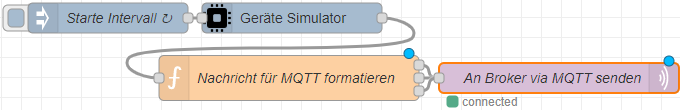
\includegraphics[width=\textwidth]{graphics/Device-Simulator-Flow.png}
\caption{Node-RED Flow des Sensorsimulators}
\label{abb:DeviceSimFlow}
\end{figure}

In \autoref{abb:DeviceSimFlow} ist ein Screenshot des Node-RED Flows zu sehen, in dem die verschiedenen Knoten, die jeweils eigene Aufgaben übernehmen, gezeigt sind. Da der Gerätesimulator die Nachrichten falsch formattiert übergibt, ist es notwendig, eigene Logik zur Reformattierung für den Transfer mit \ac{MQTT} einzusetzen. Diese ist mit einem $f$ gekennzeichnet.


